Previous phenomenological models have used truncated tensor basis expansions, with constant coefficients fit from averaging over data, to model the pressure Hessian contribution. From investigating the trained parameterization of the full expansion, we can investigate these choices.

\begin{figure}
  \centering
  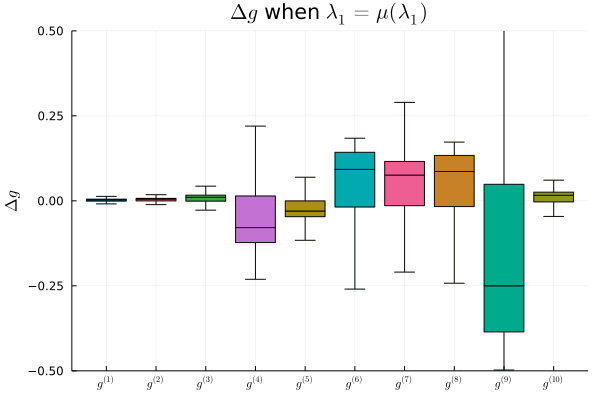
\includegraphics[width=0.5\textwidth]{./pi512/dgdl_1.png}%
  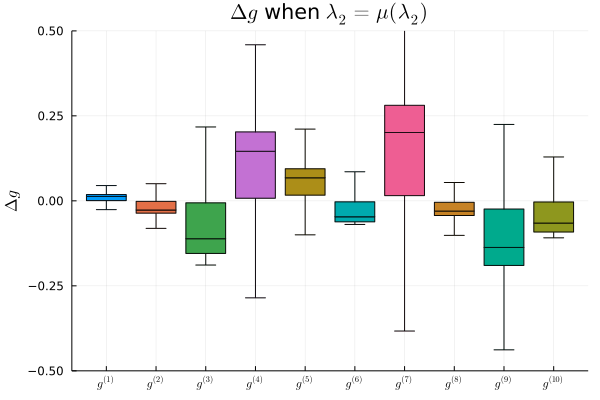
\includegraphics[width=0.5\textwidth]{./pi512/dgdl_2.png}
  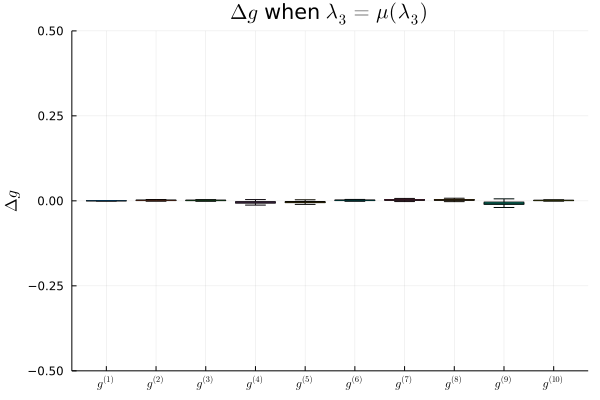
\includegraphics[width=0.5\textwidth]{./pi512/dgdl_3.png}%
  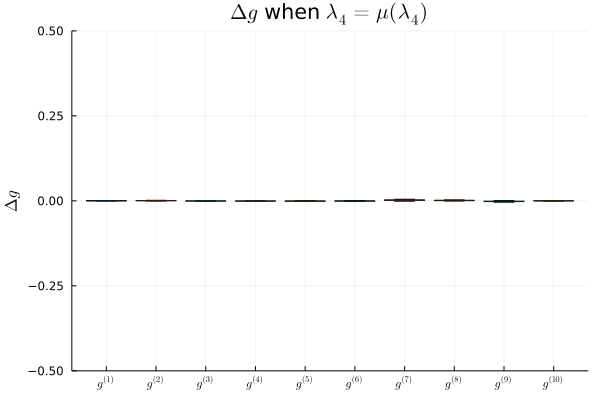
\includegraphics[width=0.5\textwidth]{./pi512/dgdl_4.png}
  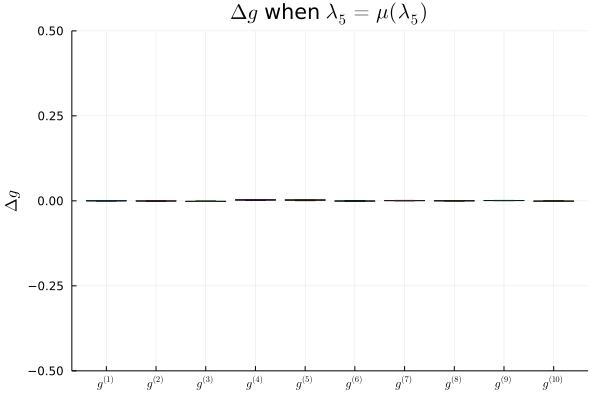
\includegraphics[width=0.5\textwidth]{./pi512/dgdl_5.png}
  \caption{ }
  \label{fig:sensitivityGs}
\end{figure}

To examine the learned model, we first investigate the sensitivity of the scalar functions $g_\theta^{(i)}$ to the variability of the invariants $\lambda_j$. This sensitivity will inform the learned ``importance'' of the $\lambda_i$ to each $g_\theta^{(i)}$. In particular, we see in figure \ref{fig:sensitivityGs} that $g^{(9)}$ has large sensitivity to changes in $\lambda_1$, while nearly no sensitivity to $\lambda_4$ or $\lambda_5$. In fact, all of the scalar functions seem to depend only on $\lambda_1, \lambda_2$. We can test this hypothesis by training a new TBNN using only the first two invariants. A comparison between the two predictions of the pressure Hessian contribution is shown in figure[\ref{fig:qrCMTComp}].

\begin{figure}
  \centering
  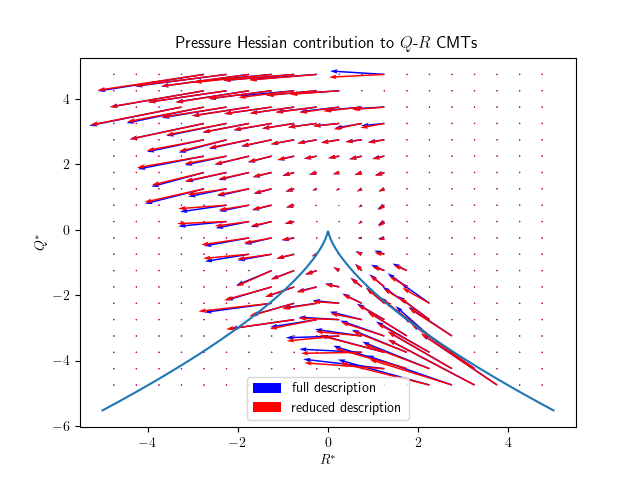
\includegraphics[width=0.75\textwidth]{./comp_qrCMT.png}
  \caption{ }
  \label{fig:qrCMTComp}
\end{figure}

We see that the change in prediction is very small - and within retraining error. Further, we can plot the $g$'s to investigate the functional dependence on the $\lambda_1,\lambda_2$, using k-nearest neighbors algorithm to interpolate between datapoints.

\begin{figure}
  \centering
  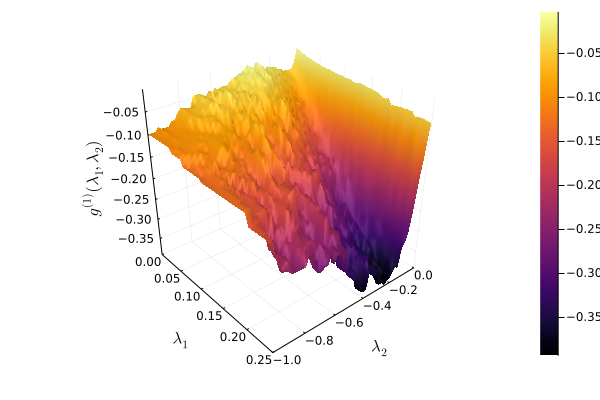
\includegraphics[width=0.33\textwidth]{./pi512/gFunctions/g1.png}%
  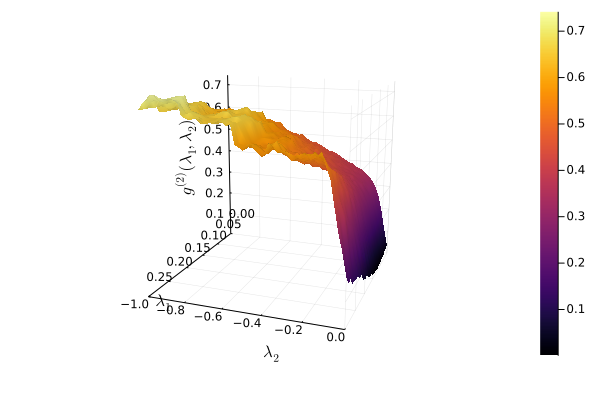
\includegraphics[width=0.33\textwidth]{./pi512/gFunctions/g2.png}%
  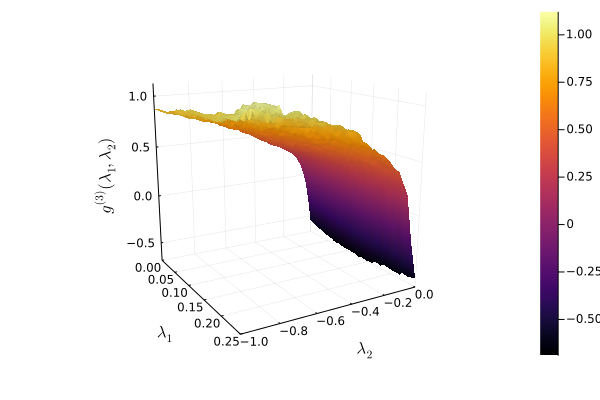
\includegraphics[width=0.33\textwidth]{./pi512/gFunctions/g3.png}
  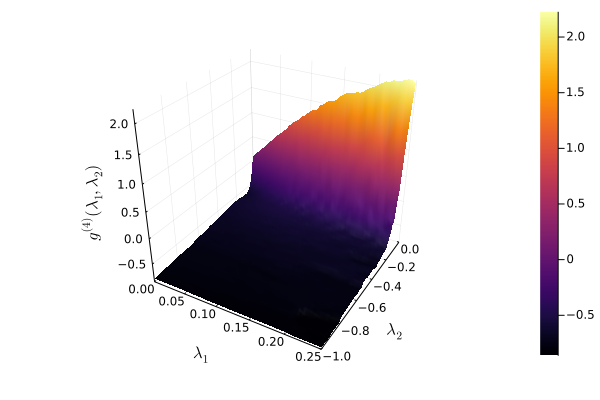
\includegraphics[width=0.33\textwidth]{./pi512/gFunctions/g4.png}%
  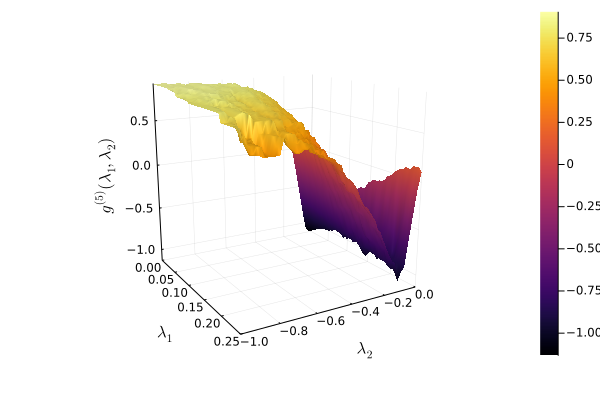
\includegraphics[width=0.33\textwidth]{./pi512/gFunctions/g5.png}%
  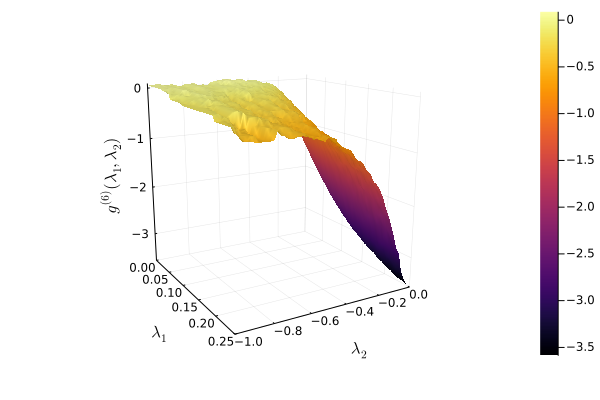
\includegraphics[width=0.33\textwidth]{./pi512/gFunctions/g6.png}
  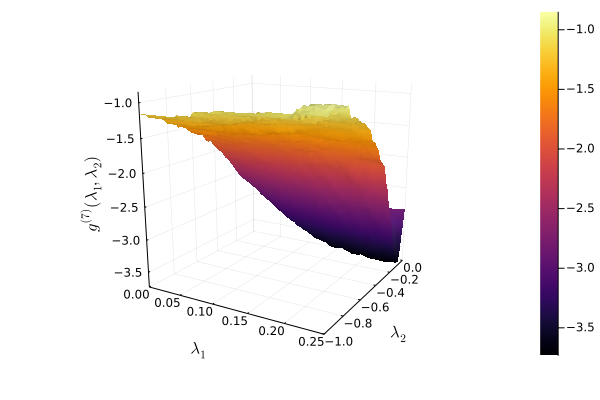
\includegraphics[width=0.33\textwidth]{./pi512/gFunctions/g7.png}%
  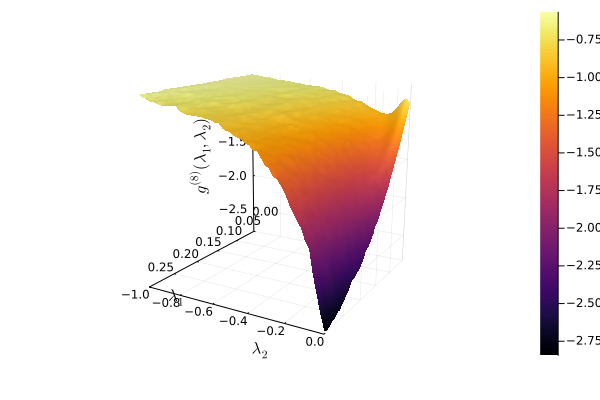
\includegraphics[width=0.33\textwidth]{./pi512/gFunctions/g8.png}%
  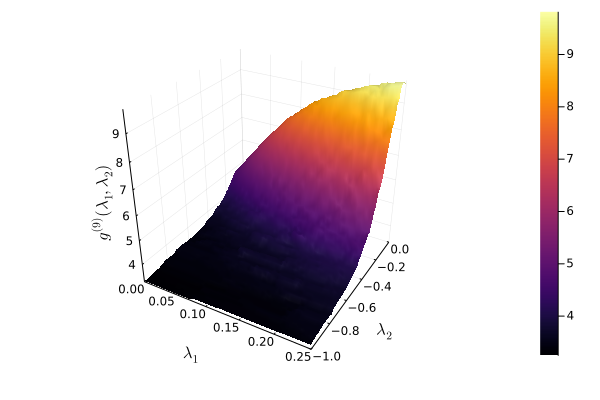
\includegraphics[width=0.33\textwidth]{./pi512/gFunctions/g9.png}
  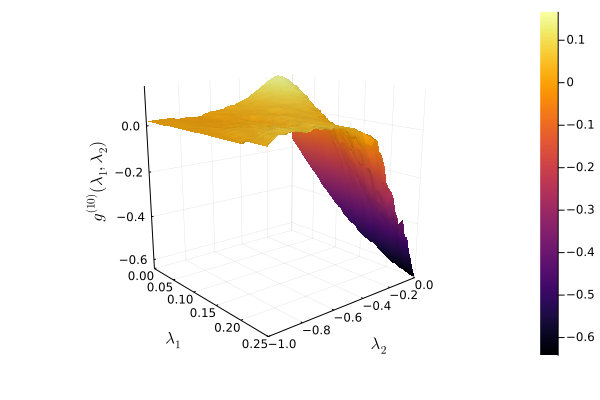
\includegraphics[width=0.33\textwidth]{./pi512/gFunctions/g10.png}%
  \caption{ }
  \label{fig:gFunctions}
\end{figure}
